\documentclass[11pt,fleqn]{article}

\usepackage{eurosym}
\usepackage{bbm}
\usepackage{pdflscape}
\usepackage{ucs}
\usepackage{psfrag,fancyhdr,layout}
\usepackage[utf8x]{inputenc}
\usepackage[english]{babel}
\usepackage[usenames,dvipsnames]{xcolor}
\usepackage{amsmath,amsthm,amsfonts}
\usepackage{geometry}
\usepackage{proba}
\usepackage{float}
\usepackage{grffile}
\usepackage{booktabs}
\usepackage{xcolor}
\usepackage{rotating}
\usepackage{enumitem}
\usepackage{multirow}
\usepackage[flushleft]{threeparttable}
\usepackage{booktabs,caption,fixltx2e}
\usepackage{soul, color}
\usepackage{graphicx}
\usepackage{caption}
\usepackage{subcaption}
\usepackage[authoryear]{natbib}

\setcounter{MaxMatrixCols}{10}


\newcommand{\nn}{\nonumber}
\newcommand{\define}{\stackrel {\Delta}{=}}
\newcommand{\bone}{\mbox {\boldmath $1$}}
\newcommand{\balpha} {\bar{\alpha}}
\newcommand{\bbeta} {\bar{\beta}}
\newcommand{\bgamma} {\bar{\gamma}}
\newcommand{\ba}{\mbox {\boldmath $a$}}
\newcommand{\bb}{\mbox {\boldmath $b$}}
\newcommand{\bB}{\mbox {\boldmath $B$}}
\newcommand{\bc}{\mbox {\boldmath $c$}}
\newcommand{\bC}{\mbox {\boldmath $C$}}
\newcommand{\bX}{\mbox {\boldmath $X$}}
\newcommand{\bD}{\mbox {\boldmath $D$}}
\newcommand{\bd}{\mbox {\boldmath $d$}}
\newcommand{\bbf}{\mbox {\boldmath $f$}}
\newcommand{\be}{\mbox {\boldmath $e$}}
\newcommand{\beps}{\mbox {\boldmath $\epsilon$}}
\newcommand{\bg}{\mbox {\boldmath $g$}}
\newcommand{\bh}{\mbox {\boldmath $h$}}
\newcommand{\cM}{{\cal{M}}}
\newcommand{\br}{\mbox {\boldmath $r$}}
\newcommand{\bu}{\mbox {\boldmath $u$}}
\newcommand{\bv}{\mbox {\boldmath $v$}}
\newcommand{\bx}{\mbox {\boldmath $x$}}
\newcommand{\tx}{\tilde{x}}
\newcommand{\tbx}{\mbox {\boldmath $\tilde{x}$}}
\newcommand{\by}{\mbox {\boldmath $y$}}
\newcommand{\bz}{\mbox {\boldmath $z$}}
\newcommand{\bI}{\mbox {\boldmath $I$}}
\newcommand{\bS}{\mbox {\boldmath $S$}}
\newcommand{\bV}{\mbox {\boldmath $V$}}
\newcommand{\bY}{\mbox {\boldmath $Y$}}
\newcommand{\bGamma}{\mbox {\boldmath $\Gamma$}}
\newcommand{\apl}{\stackrel {<}{\approx}}
\newcommand{\apg}{\stackrel {>}{\approx}}
\renewcommand{\thefootnote}{\fnsymbol{footnote}}
\newcounter{temp}
\setcounter{temp}{2}
\setcounter{footnote}{1}
\renewcommand{\thetemp}{\fnsymbol{temp}}
\renewcommand{\thesection}{\Roman{section}}
\renewcommand{\thesubsection}{\thesection-\Alph{subsection}}
\newcommand{\beq}{\begin{equation}}
\newcommand{\eeq}{\end{equation}}
\newcommand{\bea}{\begin{eqnarray}}
\newcommand{\eea}{\end{eqnarray}}
\newcommand{\denotes}{\stackrel{\triangle}{=}}
\textwidth=6.5in
\textheight=8in
\oddsidemargin=0in
\evensidemargin=0in
\topmargin=0in
\definecolor{mycol}{RGB}{0,0,80}
\newtheorem{theorem}{Theorem}
\newtheorem{acknowledgement}[theorem]{Acknowledgement}
\newtheorem{algorithm}[theorem]{Algorithm}
\newtheorem{axiom}[theorem]{Axiom}
\newtheorem{case}[theorem]{Case}
\newtheorem{claim}[theorem]{Claim}
\newtheorem{conclusion}[theorem]{Conclusion}
\newtheorem{condition}[theorem]{Condition}
\newtheorem{conjecture}[theorem]{Conjecture}
\newtheorem{criterion}[theorem]{Criterion}
\newtheorem{definition}[theorem]{Definition}
\newtheorem{example}[theorem]{Example}
\newtheorem{exercise}[theorem]{Exercise}
\newtheorem{notation}[theorem]{Notation}
\newtheorem{problem}[theorem]{Problem}
\newtheorem{proposition}[theorem]{Proposition}
\newtheorem{remark}[theorem]{Remark}
\newtheorem{solution}[theorem]{Solution}
\newtheorem{summary}[theorem]{Summary}
\newtheorem*{thm}{Theorem}
\newtheorem*{prpstn}{}
\newtheorem{lemma}{Lemma}
\renewcommand{\thelemma}{\arabic{prop1}.\arabic{lemma}}
\newtheorem{corollary}{Corollary}
\renewcommand{\thecorollary}{\arabic{theorem}.\arabic{corollary}}
\newcommand{\PE}{\mathbb{E} }
\newcounter{mycounter}
\setcounter{mycounter}{0}
\def\inprobLOW{\rightarrow_p}
\def\inprobHIGH{\,{\buildrel p \over \longrightarrow}\,}
\def\inprob{\,{\inprobHIGH}\,}
\renewcommand{\thelemma}{\arabic{prop1}.\arabic{lemma}}
\renewcommand{\thecorollary}{\arabic{theorem}.\arabic{corollary}}
\setcounter{mycounter}{0}
\def\inprobLOW{\rightarrow_p}
\def\inprobHIGH{\,{\buildrel p \over \longrightarrow}\,}
\def\inprob{\,{\inprobHIGH}\,}
\DeclareMathOperator*{\argmin}{arg\,min}
\DeclareMathOperator*{\argmax}{arg\,max}
 
\begin{document}

\title{Markov regime switching in mean and in fractional integration
parameter.}
\author{Harun Özkan\thanks{{\scriptsize Istanbul Bilgi University,
Kurtulus Deresi Caddesi, Dolapdere, Beyoglu, Istanbul, 34440, Turkey. 
\texttt{Email:~harun.ozkan@bilgi.edu.tr}}} \and Thanasis Stengos\thanks{
{\scriptsize Department of Economics, University of Guelph, 50 Stone Road
East Guelph, Ontario, Canada. \texttt{Email:~tstengos@uoguelph.ca}}. Thanasis Stengos wants to acknowledge financial assistance from NSERC of Canada. 
} \and 
Ege Yazgan\thanks{{\scriptsize Istanbul Bilgi University, Kurtulus Deresi
Caddesi, Dolapdere, Beyoglu, Istanbul, 34440, Turkey. \texttt{
Email:~ege.yazgan@bilgi.edu.tr}}} 
\thanks{{\scriptsize  We want to thank two anonymous referees for their very helpful comments on an earlier version of the paper.}} }
\maketitle

\begin{abstract}
We propose a specific general Markov-regime switching estimation both in the
long memory parameter $d $ and the mean of a time series. Following \cite%
{Tsay2009} we employ Viterbi algorithm, which combines the Viterbi
procedures, in two state Markov-switching parameter estimation. It is
well-known that existence of mean break and long memory in time series can
be easily confused with each other in most cases. Thus, we aim at observing
the deviation and interaction of mean and $d $ estimates for different cases.

A Monte Carlo experiment reveals that the finite sample performance of the
proposed algorithm for a simple mixture model of Markov-switching mean and $%
d $ changes with respect to the fractional integrating parameters and the
mean values for the two regimes.

\noindent {\small JEL Classification: C12, C22 \newline
{\ Keywords:} Markov regime switching, fractional integration, long memory
time series.}
\end{abstract}

\clearpage
\setcounter{page}{0} \thispagestyle{empty}

\renewcommand{\thesection}{\arabic{section}.} \renewcommand{\thesubsection}{%
\arabic{section}.\arabic{subsection}.} \newpage

\section{ Introduction}

The use of fractional or long memory methods has been extensive in
econometrics as they have been found to be quite effective in describing the
behavior of many macroeconomic and financial data (\cite{Lobato2000} \cite%
{Ding1993}). In particular, recent findings suggest that long memory
phenomenon is observed in LIBOR \citep{Cajueiro2005a,Cajueiro2007}, interest
rate \citep{Cajueiro2007a}, trading volume \citep{Lobato2000,Lux2007}, and
volatility of returns \citep{Lobato2000,Cajueiro2005, Granger1994} -albeit
controversial findings in terms of long memory behavior are present for the
stock returns\citep{Cajueiro2005b,Limam2003,Willinger1999}.

Similarly, since the seminal work of Hamilton (1989) 
% write the cite{Hamilton1989} version here.
the Markov--switching model has been a popular vehicle to analyze economic
phenomena that are likely to obey regime changes. Recently, \cite{Tsay2009}
(hereafter TH) has combined the two approaches in a unified framework by
introducing a Markov-switching-ARFIMA (MS-ARFIMA) process which extends the
hidden Markov model with a latent state variable, allowing for the different
regimes to have different degrees of long memory. Recent papers in the
literature have been concerned with changes in the persistence of a
univariate time series, considering primarily a shift from a unit root
process [$I(1) $] to a stationary process [$I(0) $] or vice versa at some
unknown date over the sample under consideration. In that strand of the
literature the analysis centers on the properties of estimators (and tests)
in these extreme cases, see \cite{Perron2006} for a survey of testing
procedures and \cite{Chong2001} and \cite{Kejriwal2010} for some recent
results on the properties of the break estimators. These models however deal
with the extreme dichotomy of [$I(1)] $ versus [$I(0) $] and do not allow
for long memory and fractional integration.

Models that allow for different long memory regimes have been used in the
literature but the regime switching is forced by an observable state
variable as opposed to the latent nature of the state variable in the
MS--ARFIMA model, see \cite{Haldrup2006}. The main motivation behind the TH
MS--ARFIMA model has been the observation by \cite{Diebold2001} that a
mixture model of latent Markov-switching mean can generate long memory
dependence. In other words, structural change and long memory may be easily
confused in estimation. Hence, the main emphasis of the TH approach\ has
been to disentangle the impact of long memory dependence on the estimates of
the latent regime parameters in the MS--ARFIMA framework. It is worth noting
that in this context the direct application of the EM algorithm used by \cite%
{Hamilton1989} and \cite{Hamilton1990} is not applicable due to the
non-Markovian nature of the model. One of the main contributions of TH is
the use of the Viterbi algorithm to estimate the MS--ARFIMA model. This
algorithm is capable of tackling the hidden Markov process observed in a
general ARFIMA framework, something that is not generally possible with the
EM algorithm. The algorithm discussed above is not the only choice
practically available in estimation of the parameters of Markov regime
switching model. Other widely used algorithms are, for example, the
forward-backward algorithm, the Baum-Welch algorithm and the BCJR algorithm.
The forward-backward algorithm is an inference algorithm for hidden Markov
models which computes the posterior marginals of all hidden state variables
given a sequence of observations. The Baum-Welch algorithm is a special
forward-backward algorithm and also relies on EM algorithm. The BCJR
algorithm, also called Maximum posteriori probability (MAP) decoder, named
after \cite{Bahl:1974}, relies on maximization of posteriori probabilities.
These algorithm has several modified and tailored versions\footnote{%
Examining the performance of these other algorithms is beyond the scope of
the present note and is left for future research.}. 

However, the TH analysis did not consider regime switching in the
long memory parameter but only in the mean both in their simulations and
their empirical application. Yet long memory parameter regime switching may
have similar contamination effects on the estimation of the mean parameters
as it would be the case in the opposite case considered by TH. This
possibility in fact was indicated by \cite{Diebold2001} concern mentioned
above. In this note we explicitly consider the case where the long memory
parameter may be subject to regime switching, while the mean can be
unchanging or regime switching itself. By allowing the direct impact of long
memory regime switching on the mean parameters (whether in regime switching
mode or not) would allow us to asses the possible contamination and impact
that such long memory structural break may have on the mean estimates. We
conduct a Monte Carlo simulation that considers contamination to be going
both ways between mean and long memory parameter breaks. Our results suggest
that in addition to the findings by TH that only considered breaks in the
mean parameter, breaks in the long memory parameter can have similar effects
on the (in sample) fitting ability of the model irrespective of the presence
of breaks in the mean parameter, confirming the contamination concern raised
by \cite{Diebold2001}.

The rest of the paper is organized as follows. In the next section we
present the model that we analyze as well as the Viterbi algorithm we use following
TH. We then proceed to present our simulations that analyze the possible
contamination that could run from long memory parameter breaks to mean
parameter breaks and vice-versa. Finally we conclude.

\section{Viterbi maximum likelihood EM algorithm}

Consider the fractionally integrated process $y_{t}$ defined as 
\begin{equation}
\left( 1-L\right) ^{d}y_{t}=\mu +\varepsilon _{t}  \label{eq:fi}
\end{equation}%
where $\varepsilon _{t}$ is white noise, $L$ is the lag operator, $d$ is the
fractional integration parameter and $\mu $ is real valued drift.

Let $y_{1}=0$ and $\hat{y}=\phi _{t1}y_{t-1}+\ldots +\phi _{t1}y_{1}$ be the
one-step predictors of the process {$y_{t}$}. The coefficients has the
following recursive structure: 
\begin{eqnarray}
\phi _{tt} &=&\left[ \gamma (t)-\sum\limits_{i=1}^{t-1}\gamma (t-i)\right]
\nu _{t-1}  \notag \\
\phi _{tj} &=&\phi _{tj}-\phi _{tt}\phi _{t-1t-j},\qquad j=1,\ldots ,T-1 \\
\nu _{tj} &=&\nu _{t-1}(1-\phi _{tt}^{2}),\qquad \quad t=1,\ldots ,T-1 
\notag
\end{eqnarray}%
where $\gamma (t)$ is the autocovariance function of order $t$, $\nu
_{0}=\gamma _{0}$. In a fractionally integrated processes such as specified
in Equation \ref{eq:fi}, we have 
\begin{equation*}
\gamma (t)=\dfrac{\Gamma (1-2d)\Gamma (d-t)}{\Gamma (d)\Gamma (1-d)\Gamma
(1-d-t)}
\end{equation*}%
where $\Gamma (x)$ is the gamma function.

Defining the prediction error $e_t=y_t - \hat{y}_t $, then $e_t = Ly $ where 
$L $ is

\begin{equation}
\begin{bmatrix}
1 & 0 & 0 & \dots & 0 \\ 
-\phi_{11} & 1 & 0 & \dots & 0 \\ 
-\phi_{22} & -\phi_{21} & 1 & \dots & 0 \\ 
\vdots & \vdots & \vdots & \ddots & \vdots \\ 
-\phi_{T-1 T-1} & -\phi_{T-1 T-2} & -\phi_{T-1 T-3} & \dots & 1%
\end{bmatrix}
\label{eq:lev}
\end{equation}
Setting $\Gamma_\theta =LDL^{\prime }$, where $D $ is diagonal matrix with $%
diag(\nu_0,\ldots,\nu_{T-1}) $, we have $\det\Gamma_\theta= \prod_{j=1}^{n}
\nu_{j-1}$. Consequently, $Y^{\prime }\Gamma_\Theta^{-1} Y=e^{\prime -1}e$,
where $Y=(y_1,\ldots,y_T) $ and $e_t= y_t-\hat{y}_t$. Then, the
log-likelihood function may be written as 
\begin{equation}
\mathcal{L} (\theta) = -\dfrac{1}{2}\sum\limits_{t=1}^{T}\log\nu_{t-1} -%
\dfrac{1}{2}\sum\limits_{t=1}^{T} \dfrac{e^2_t}{\nu_{t-1}}
\end{equation}
for the model specified in Equation \ref{eq:fi}.

Now, we consider a $2 -$state homogeneous Markov chain $S_t $ taking values
1 or 2. Let ${S_t}^T_{t=1} $ be the latent sample path of the Markov chain.
At each time point $t $, $S_t $ can assume only an integer value of 1 or 2,
and its transition probability matrix is 
\begin{equation}
\mathcal{P} = \left[ 
\begin{matrix}
p_{11} & p_{12} \\ 
p_{21} & p_{22}%
\end{matrix}
\right]
\end{equation}
where $p_{ij} = \P (S_{t} = j \, | \, S_{t-1} = i) $ and $p_{i1}+p_{i2}=1 $
for $i=1,2 $.

We specify the corresponding regime switching fractionally integrated
process as 
\begin{equation}
\left( 1-L\right) ^{d^{s_{t}}}y_{t}=\mu ^{s_{t}}+\varepsilon _{t}^{s_{t}}
\end{equation}
with the unobserved state vector $S=(s_t)_{1 \leq t\leq T} $.

In this study, we are going to employ the Viterbi algorithm to estimate the
unobserved state vector.$S$. The Viterbi algorithm is forward decoding
procedure widely used in signal processing problems with Hidden Markov
Models (HMM) specification. The main idea behind this algorithm is to
\textquotedblleft decode" the sequence of states $s_{t}$ in the Markov chain
iteratively starting from time $1$ to $T$. Given the previous state, $%
s_{t-1} $, and the unconditional likelihood function for the observations up
to $t$, $(y_{s})_{0\leq s\leq t}$ and a parameter vectors $\xi _{1}$ and $%
\xi _{2}$, it enables us to choose the most probable state at $t$, i.e., $%
s_{t}$.

In particular, specifiying the unconditional likelihood functions for both
states at $t $ as 
\begin{equation}
l^j_t = \frac{1}{\sqrt{2 \pi} \sigma_{j}} e^{-\frac{ (y_{t}-\hat{y}%
^{(j)}_{t})^2}{2 \sigma_{j}^2}}
\end{equation}
where $\hat{y}^{(j)}_t=\hat{y}^{(1)}_t(\xi_j, \ (y_u)_{1 \leq u\leq t})$ and 
$\xi_j= (\mu_j, d_j,\sigma_j,) $, $j=1,2 $ and it can be calculated by $Ly+y 
$ . Given the likelihood function,, the parameter vectors $\xi^j $, and the
transition probabilities $P $, by Viterbi specification we can iteratively
estimate the path of the states $s_t $ as follows: 
\begin{equation}
\mathcal{S}_t= \argmax \limits_{s_t \in \{1,2\}}( l^{s_t}_t P(s_t|\mathcal{S}%
_{t-1}))
\end{equation}
given $s_0 $ and the initial probabilities $\pi_j = \mathbb{P}(s_0=j)$, and $%
\hat{y_0} $, where $\mathcal{S_t} $ is the Viterbi decoded state at $t $.

Then, the estimation of parameter vectors $\xi_j $ and the transition
probabilities $p_{ij} $ is obtained by maximixzing the following
log-likelihood function:

\begin{equation}
\mathcal{L}(\xi _{1},\xi _{2},y)=-\dfrac{1}{2}\sum\limits_{t=1}^{T}\log
\sigma _{j}-\dfrac{1}{2}\sum\limits_{t=1}^{T}\dfrac{e_{t}^{2}}{\sigma _{j}}%
+\sum\limits_{t=1}^{T}\mathbb{P}(\mathcal{S}_{t}|\mathcal{S}_{t-1})
\label{eq:finalLikelihood}
\end{equation}
{The computational complexity of this maximization is $\mathcal{O}(n^{2})$.
In comparison, the EM algorithm of Hamilton (1989), which is exhaustively
used in estimation of Markov regime switching models, cannot be employed in
this case (when $d$ is allowed to be state depended) for one main reason:
the number of possible state paths the EM algorithm is going to account for
is $n^{T}$ (since $n=2$ in our case, it is $2^{T}$, hence, implying a
computational complexity of $O(2^{T})$. Thus, EM is computationally much
more demanding in comparison to Viterbi algorithm, which is $\mathcal{O}%
(n^{2})$ in computational complexity. Furthermore, \cite{Tsay2008} argues, that
the model we examine above  \textquotedblleft \ldots\ cannot be written in a
state-space form due to the presence of a fractional differencing parameter,
implying that we cannot apply the EM algorithm considered in Hamilton (1990)
\ldots\ because the non-Markovian nature of the model prevents us from using
the results in (4.2) of Hamilton (1990)\textquotedblright\ (\citealp{Tsay2008},
page. 3).

TH made a similar argument that the EM algorithm proposed by Hamilton (1989)
is unstable for estimating the Markov regime switching $d$. We confirmed
that by conducting a small scale computation exercise using the EM algorithm%
\footnote{%
However, , we made a na\"{\i}ve experiment to estimate $d_{s_{t}}$ by
Hamilton (1989) method, for a series generated by the process $\left(
1-L\right) ^{d^{s_{t}}}y_{t}=\mu ^{s_{t}}+\varepsilon _{t}$ with the true
values of $d_{1}=0,d_{2}=0.5,\mu _{1}=0,\mu _{2}=0$ and $\varepsilon
_{t}\sim iidN(0,0.25)$. We obtained $\widehat{d_{1}}=0.142,\widehat{d_{2}}%
=0.411,\widehat{\mu }_{2}=-0.12,\widehat{\mu }_{2}=0.42,$ and $\sigma
_{\varepsilon _{t}}^{2}=0.32$. From a computational perspective, it also
took much longer to compute the estimators than the Viterbi algorithm did; with a
2.7 GHz i7 single thread processor it takes 1.8 times longer time than that
of the Viterbi algorithm computation.}.

In the context of the present model, even though the log-likelihood function given by Equation \ref{eq:finalLikelihood}, is well-defined, the properties of the estimators of the long-memory parameter and the mean level under regime switching are not derived. We conjecture that an analytical derivation of the asymptotic distribution of these estimators might entail an analytical framework such as \cite{Hansen2000}.

We now proceed with the application of the Viterbi algorithm in a Monte
Carlo simulation where we will study breaks in both long memory and mean
parameters.


\section{The Monte Carlo experiment}

The Monte Carlo experiments that we conduct in this note is to consider the
simplest possible framework of analysis an MS-ARFIMA $(0,d,0)$ to do the
analysis as we are interested in isolating the effects of spillovers between
the  regime shifts of the two simple parameters in the model, $\mu $ and $%
d.$ We carry out the Monte Carlo experiment for the Cartesian product space $%
\mu _{1}\times \mu _{2}\times d_{1}\times d_{2}$ of true $\mu _{1},\mu
_{2},d_{1},d_{2}$ vales such that $\mu _{i}\in \{0,0.5,1.0\}$, $d_{i}\in
\{-0.50,0.00,0.25,0.50,0.75,1.00\}$ for $i=1,2$.

First, we generated the series $y_{t}$ 
\begin{equation*}
\left( 1-L\right) ^{d^{s_{t}}}y_{t}=\mu ^{s_{t}}+\varepsilon _{t}
\end{equation*}%
where $s_{t}=1$ if $t\leq T/2$ and $2$ otherwise; $\varepsilon _{t}$ are $%
iid $ and distributed $N(0,0.25)$; $T$ is 256. $d_{1},d_{2},\mu _{1}$, and $%
\mu _{2}$ are selected such that $d_{i}\in
\{-0.50,0.00,0.25,0.50,0.75,1.00\} $, $\mu _{i}\in \{0.0,0.5,1.0\}$ for $%
i=1,2$.

Then, we obtain the estimates of $\widehat{d_{1}},\widehat{d_{2}},\widehat{%
\mu }_{2},\widehat{\mu }_{2}$, and $\widehat{\sigma _{\varepsilon }}_{t}$
values by the procedure described above. We conduct 1000 replications for
the $(d_{1},d_{2},\mu _{1},\mu _{2})$ quadruple. 

The results are presented in Tables 1 to 4 and Figure 1. Table 1 simply
presents the average parameter estimates over the total number of
replications, Table 2 presents the root mean square errors for the parameter
estimates, Table 3 the mean absolute biases and finally Table 4 the in
sample root mean squared errors of the model fit. The results of Table 4 are
best seen in Figure 1 and it becomes clear that whether there is a break in
the mean (different values of $\mu _{1},\mu _{2}$) or not the model fit
seems to be unaffected (as measured by the root mean squared error). In
other words we observe that structural breaks in the long memory parameter
produce similar in sample estimation patterns irrespective of the presence
of breaks in the mean parameter. Hence, these results confirm the original
concern raised by \cite{Diebold2001}, something that was not possible to be
seen in the work of TH who only considered in his simulation study breaks in
the mean but not in the long memory parameter $d.$ The upshot of our
analysis is that one has to be careful in claiming the occurrence of
structural breaks in such models as the presence of such breaks may be
difficult to disentangle. For that purpose one would need to develop more
appropriate joint testing procedures that would be able to discern the
nature of possible such breaks. The results also confirm that as $d$, 
the long memory parameter gets close to unity, the estimates of
the mean level parameter $\mu $ tend to become inconsistent as
expected in the presence of unit roots.

\section{Conclusion}

In this note we consider a general Markov-regime switching estimation both
in the long memory parameter $d$ and the mean of a time series. Following 
\cite{Tsay2009} we employ the Viterbi algorithm in a two state
Markov-switching parameter estimation. Since it has been suggested in the
literature that mean and long memory parameter breaks in time series can be
easily confused with each other \cite{Diebold2001}, our aim is to produce
evidence for this assertion by means of a Monte Carlo simulation that
considers both breaks in both the mean and the long memory parameters. Our
results confirm the above assertion, since we observe that structural breaks
in the long memory parameter produce similar in sample estimation patterns
irrespective of the presence of breaks in the mean parameter. Our results
are complementary to TH who only considers breaks in the mean parameter in
his simulation study. Our results call for the development for joint tests
that would be able to discern the nature of possible such breaks. 
However, given the results of our analysis there are many outstanding issues
that we leave for future research. First, a more comprehensive Monte Carlo
simulation study would need to allow for a more general MS-ARFIMA $(p,d,q)$%
structure. Furthermore, one would need to investigate the
asymptotic properties of the estimators of $\mu $ and $d$%
 we obtain under regime switching. Even though the likelihood
function is well defined, in the context of unknown breaks, we conjecture
that  one would need to use a framework that is used in threshold models
with unknown thresholds, see \cite{Hansen2000}. An investigation of such a
problem is beyond the scope of this paper and is left for future research.  

\bibliographystyle{chicago}
\bibliography{bibMarkovd}
\clearpage

\begin{landscape}
	
	\begin{table}[!ht]
		
		\section*{Tables and Figures}
		\centering
		\caption{True parameters and estimated parameters by the Monte Carlo study.}
		\begin{tabular}{|r|rrrr|rrrr|rrrr|}
			\hline
			\multicolumn{1}{|c|}{\multirow{2}[4]{*}{$ d $}} & \multicolumn{4}{c|}{$ (\mu_1,\mu_2)=(0,0)$}    & \multicolumn{4}{c|}{$ (\mu_1,\mu_2)=(0,0.5)$}  & \multicolumn{4}{c|}{$ (\mu_1,\mu_2)=(0,1)$} \\
			\cline{2-13}    \multicolumn{1}{|c|}{} & \multicolumn{1}{c}{$ d_1 $} & \multicolumn{1}{c}{$ d_2$} & \multicolumn{1}{c}{$\mu_1$} & \multicolumn{1}{c|}{$ \mu_2 $} & \multicolumn{1}{c}{$d_1$} & \multicolumn{1}{c}{$d_2$} & \multicolumn{1}{c}{$\mu_1$} & \multicolumn{1}{c|}{$\mu_2$} & \multicolumn{1}{c}{$ d_1 $} & \multicolumn{1}{c}{$d_2$} & \multicolumn{1}{c}{$\mu_1$} & \multicolumn{1}{c|}{$\mu_2$} \\
			\hline
			(-0.5,-0.5) & 0.080 & -0.344 & -0.083 & 0.011 & -0.505 & -0.335 & -0.042 & 0.563 & -0.472 & -0.363 & 0.032 & 0.918 \\
			(-0.5, 0) & -0.566 & -0.156 & -0.065 & 0.149 & -0.407 & -0.161 & 0.099 & 0.532 & -0.172 & 0.068 & 0.015 & 0.905 \\
			(-0.5, 0.25) & -0.518 & -0.235 & -0.095 & 0.158 & -0.455 & -0.161 & 0.099 & 0.545 & -0.472 & 0.078 & 0.015 & 0.905 \\
			(-0.5, 0.5) & -0.580 & 0.530 & -0.135 & 0.003 & -0.627 & 0.445 & -0.014 & 0.524 & -0.595 & 0.388 & 0.013 & 0.896 \\
			(-0.5, 0.75) & -0.510 & 0.730 & -0.091 & 0.003 & -0.627 & 0.725 & -0.014 & 0.558 & -0.595 & 0.788 & 0.010 & 0.913 \\
			(-0.5, 1) & -0.415 & 0.906 & 0.047 & 0.172 & -0.338 & 1.080 & 0.161 & 0.717 & -0.466 & 0.844 & -0.017 & 1.036\\
			\hline
			(0.0, 0.0) & -0.096 & -0.017 & -0.240 & -0.024 & -0.256 & 0.141 & -0.079 & 0.562 & -0.109 & 0.095 & -0.057 & 0.880 \\
			(0.0, 0.25) & -0.106 & -0.252 & -0.014 & 0.008 & 0.144 & 0.254 & -0.079 & 0.562 & 0.110 & 0.245 & -0.055 & 0.895 \\
			(0.0, 0.5) & 0.028 & 0.425 & -0.082 & -0.099 & 0.015 & 0.496 & -0.111 & 0.594 & 0.108 & 0.553 & -0.004 & 0.927 \\
			(0.0, 0.75) & 0.017 & 0.785 & -0.082 & -0.099 & 0.115 & 0.725 & -0.111 & 0.524 & 0.095 & 0.714 & -0.074 & 0.927 \\
			(0.0, 1.0) & 0.058 & 1.008 & 0.127 & -0.071 & 0.282 & 0.963 & -0.175 & 0.573 & 0.041 & 0.971 & -0.094 & 1.387 \\
			\hline
			(0.5, 0.5) & 0.524 & 0.518 & -0.136 & 0.056 & 0.542 & 0.536 & -0.074 & 0.529 & 0.448 & 0.549 & 0.089 & 1.207 \\
			(0.5, 0.75) & 0.556 & 0.768 & -0.106 & 0.046 & 0.552 & 0.752 & -0.074 & 0.519 & 0.476 & 0.746 & 0.029 & 1.207 \\
			(0.5, 1) & 0.465 & 0.934 & -0.140 & 0.213 & 0.528 & 1.036 & -0.071 & 0.528 & 0.513 & 1.132 & -0.013 & 1.155 \\
			\hline
			(.25,1) & 0.235 & 0.964 & -0.119 & 0.115 & 0.215 & 1.014 & -0.073 & 0.582 & 0.234 & 1.175 & -0.053 & 1.154 \\
			(.75,1) & 0.765 & 0.957 & -0.136 & 0.103 & 0.765 & 1.217 & -0.071 & 0.608 & 0.713 & 1.107 & -0.031 & 1.168 \\
			(1, 1) & 1.149 & 1.188 & -0.015 & -0.232 & 0.826 & 1.004 & 0.082 & 0.681 & 0.950 & 1.198 & -0.139 & 0.996 \\
			\hline
		\end{tabular}
		\label{tab:1}
	\end{table}
	
	\newpage
	
	% Table generated by Excel2LaTeX from sheet 'Absolute estimation error'
	\begin{table}[htbp]
		\centering
		\caption{Root mean squared errors for the parameters computed as $ \sqrt{N^{(-1)}\sum_{i}^{N}(\widehat{x_i}-x)^2} $ where $ x $ may be  $d_1,d_2,\mu_1, \mu_2$}.
		\begin{tabular}{|r|rrrr|rrrr|rrrr|}
			\hline
			\multicolumn{1}{|c|}{\multirow{2}[4]{*}{$ d $}} & \multicolumn{4}{c|}{$ (\mu_1,\mu_2)=(0,0)$}    & \multicolumn{4}{c|}{$ (\mu_1,\mu_2)=(0,0.5)$}  & \multicolumn{4}{c|}{$ (\mu_1,\mu_2)=(0,1)$} \\
			\cline{2-13}    \multicolumn{1}{|c|}{} & \multicolumn{1}{c}{$ d_1 $} & \multicolumn{1}{c}{$ d_2$} & \multicolumn{1}{c}{$\mu_1$} & \multicolumn{1}{c|}{$ \mu_2 $} & \multicolumn{1}{c}{$d_1$} & \multicolumn{1}{c}{$d_2$} & \multicolumn{1}{c}{$\mu_1$} & \multicolumn{1}{c|}{$\mu_2$} & \multicolumn{1}{c}{$ d_1 $} & \multicolumn{1}{c}{$d_2$} & \multicolumn{1}{c}{$\mu_1$} & \multicolumn{1}{c|}{$\mu_2$} \\
			\hline
			(-0.5,-0.5) & 0.580 & 0.156 & 0.083 & 0.011 & 0.005 & 0.165 & 0.042 & 0.063 & 0.028 & 0.137 & 0.032 & 0.082 \\
			(-0.5, 0) & 0.066 & 0.156 & 0.065 & 0.149 & 0.093 & 0.161 & 0.099 & 0.032 & 0.328 & 0.068 & 0.015 & 0.095 \\
			(-0.5, 0.25) & 0.018 & 0.485 & 0.095 & 0.158 & 0.045 & 0.411 & 0.099 & 0.045 & 0.028 & 0.172 & 0.015 & 0.095 \\
			(-0.5, 0.5) & 0.080 & 0.030 & 0.135 & 0.003 & 0.127 & 0.055 & 0.014 & 0.024 & 0.095 & 0.112 & 0.013 & 0.104 \\
			(-0.5, 0.75) & 0.010 & 0.020 & 0.091 & 0.003 & 0.127 & 0.025 & 0.014 & 0.058 & 0.095 & 0.038 & 0.010 & 0.087 \\
			(-0.5, 1) & 0.085 & 0.094 & 0.047 & 0.172 & 0.162 & 0.080 & 0.161 & 0.217 & 0.034 & 0.156 & 0.017 & 0.036 \\
			\hline
			(0.0, 0.0) & 0.096 & 0.017 & 0.240 & 0.024 & 0.256 & 0.141 & 0.079 & 0.062 & 0.109 & 0.095 & 0.057 & 0.120 \\
			(0.0, 0.25) & 0.106 & 0.502 & 0.014 & 0.008 & 0.144 & 0.004 & 0.079 & 0.062 & 0.110 & 0.005 & 0.055 & 0.105 \\
			(0.0, 0.5) & 0.028 & 0.075 & 0.082 & 0.099 & 0.015 & 0.004 & 0.111 & 0.094 & 0.108 & 0.053 & 0.004 & 0.073 \\
			(0.0, 0.75) & 0.017 & 0.035 & 0.082 & 0.099 & 0.115 & 0.025 & 0.111 & 0.024 & 0.095 & 0.036 & 0.074 & 0.073 \\
			(0.0, 1.0) & 0.058 & 0.008 & 0.127 & 0.071 & 0.282 & 0.037 & 0.175 & 0.073 & 0.041 & 0.029 & 0.094 & 0.387 \\
			\hline
			(0.5, 0.5) & 0.024 & 0.018 & 0.136 & 0.056 & 0.042 & 0.036 & 0.074 & 0.029 & 0.052 & 0.049 & 0.089 & 0.207 \\
			(0.5, 0.75) & 0.056 & 0.018 & 0.106 & 0.046 & 0.052 & 0.002 & 0.074 & 0.019 & 0.024 & 0.004 & 0.029 & 0.207 \\
			(0.5, 1) & 0.035 & 0.066 & 0.140 & 0.213 & 0.028 & 0.036 & 0.071 & 0.028 & 0.013 & 0.132 & 0.013 & 0.155 \\
			\hline
			(.25,1) & 0.015 & 0.036 & 0.119 & 0.115 & 0.035 & 0.014 & 0.073 & 0.082 & 0.016 & 0.175 & 0.053 & 0.154 \\
			(.75,1) & 0.015 & 0.043 & 0.136 & 0.103 & 0.015 & 0.217 & 0.071 & 0.108 & 0.037 & 0.107 & 0.031 & 0.168 \\
			(1, 1) & 0.149 & 0.188 & 0.015 & 0.232 & 0.174 & 0.004 & 0.082 & 0.181 & 0.050 & 0.198 & 0.139 & 0.004 \\
			\hline
		\end{tabular}
		\label{tab:2}
	\end{table}
	
	\newpage

	\begin{table}[htbp]
		\centering
		\caption{Absolute estimation errors computed as $ N^{(-1)}\sum_{i}^{N}|\widehat{x_i}-x |$ where $ x $ is  $d_1,d_2,\mu_1, \mu_2$.}
		\begin{tabular}{|r|rrrr|rrrr|rrrr|}
			\hline
			\multicolumn{1}{|c|}{\multirow{2}[4]{*}{$ d $}} & \multicolumn{4}{c|}{$ (\mu_1,\mu_2)=(0,0)$}    & \multicolumn{4}{c|}{$ (\mu_1,\mu_2)=(0,0.5)$}  & \multicolumn{4}{c|}{$ (\mu_1,\mu_2)=(0,1)$} \\
			\cline{2-13}    \multicolumn{1}{|c|}{} & \multicolumn{1}{c}{$ d_1 $} & \multicolumn{1}{c}{$ d_2$} & \multicolumn{1}{c}{$\mu_1$} & \multicolumn{1}{c|}{$ \mu_2 $} & \multicolumn{1}{c}{$d_1$} & \multicolumn{1}{c}{$d_2$} & \multicolumn{1}{c}{$\mu_1$} & \multicolumn{1}{c|}{$\mu_2$} & \multicolumn{1}{c}{$ d_1 $} & \multicolumn{1}{c}{$d_2$} & \multicolumn{1}{c}{$\mu_1$} & \multicolumn{1}{c|}{$\mu_2$} \\
			\hline
			(-0.5,-0.5) & 0.580 & 0.158 & 0.130 & 0.101 & 0.025 & 0.166 & 0.107 & 0.119 & 0.035 & 0.139 & 0.104 & 0.132 \\
			(-0.5, 0) & 0.070 & 0.157 & 0.119 & 0.179 & 0.096 & 0.163 & 0.141 & 0.107 & 0.328 & 0.072 & 0.097 & 0.138 \\
			(-0.5, 0.25) & 0.029 & 0.485 & 0.139 & 0.188 & 0.053 & 0.412 & 0.140 & 0.112 & 0.035 & 0.173 & 0.103 & 0.139 \\
			(-0.5, 0.5) & 0.084 & 0.036 & 0.170 & 0.101 & 0.129 & 0.058 & 0.100 & 0.102 & 0.098 & 0.116 & 0.098 & 0.145 \\
			(-0.5, 0.75) & 0.025 & 0.032 & 0.134 & 0.102 & 0.129 & 0.034 & 0.099 & 0.114 & 0.098 & 0.045 & 0.100 & 0.133 \\
			(-0.5, 1) & 0.088 & 0.096 & 0.111 & 0.199 & 0.163 & 0.083 & 0.188 & 0.239 & 0.040 & 0.158 & 0.102 & 0.107 \\
			\hline
			(0.0, 0.0) & 0.101 & 0.032 & 0.260 & 0.104 & 0.257 & 0.143 & 0.129 & 0.115 & 0.111 & 0.098 & 0.116 & 0.157 \\
			(0.0, 0.25) & 0.108 & 0.502 & 0.101 & 0.100 & 0.146 & 0.028 & 0.128 & 0.114 & 0.113 & 0.022 & 0.115 & 0.146 \\
			(0.0, 0.5) & 0.037 & 0.081 & 0.127 & 0.139 & 0.030 & 0.021 & 0.150 & 0.135 & 0.110 & 0.057 & 0.098 & 0.125 \\
			(0.0, 0.75) & 0.031 & 0.041 & 0.130 & 0.140 & 0.117 & 0.045 & 0.151 & 0.105 & 0.098 & 0.042 & 0.124 & 0.123 \\
			(0.0, 1.0) & 0.062 & 0.025 & 0.161 & 0.125 & 0.283 & 0.050 & 0.202 & 0.124 & 0.047 & 0.039 & 0.136 & 0.400 \\
			\hline
			(0.5, 0.5) & 0.035 & 0.029 & 0.168 & 0.114 & 0.048 & 0.043 & 0.127 & 0.107 & 0.059 & 0.053 & 0.133 & 0.229 \\
			(0.5, 0.75) & 0.062 & 0.028 & 0.147 & 0.112 & 0.057 & 0.023 & 0.126 & 0.104 & 0.035 & 0.021 & 0.106 & 0.229 \\
			(0.5, 1) & 0.042 & 0.070 & 0.172 & 0.232 & 0.038 & 0.047 & 0.122 & 0.104 & 0.030 & 0.135 & 0.097 & 0.185 \\
			\hline
			(.25,1) & 0.027 & 0.043 & 0.156 & 0.153 & 0.041 & 0.026 & 0.124 & 0.130 & 0.025 & 0.177 & 0.111 & 0.184 \\
			(.75,1) & 0.029 & 0.050 & 0.168 & 0.141 & 0.026 & 0.218 & 0.125 & 0.148 & 0.043 & 0.110 & 0.103 & 0.197 \\
			(1, 1) & 0.151 & 0.190 & 0.097 & 0.252 & 0.175 & 0.021 & 0.124 & 0.208 & 0.053 & 0.199 & 0.171 & 0.097 \\
			\hline
		\end{tabular}
		\label{tab:3}
	\end{table}
\end{landscape}

% Table generated by Excel2LaTeX from sheet 'RMSE_y'
\begin{table}[!h]
\caption{In-sample {mean squared errors}}
\label{tab:4}\centering
\begin{tabular}{|r|r|c|c|c|}
\hline
Cases & $(d_1, d_2) $ & \multicolumn{1}{c|}{$(\mu_1,\mu_2)=(0,0) $} & 
\multicolumn{1}{c|}{$(\mu_1,\mu_2)=(0, 0.5) $} & \multicolumn{1}{c|}{$%
(\mu_1,\mu_2)=(0,1) $} \\ \hline
1 & (-0.5,-0.5) & 0.2582 & 0.3142 & 0.3573 \\ 
2 & (-0.5, 0) & 0.1879 & 0.1247 & 0.1611 \\ 
3 & (-0.5, 0.25) & 0.3402 & 0.2915 & 0.3296 \\ 
4 & (-0.5, 0.5) & 0.3960 & 0.3810 & 0.2860 \\ 
5 & (-0.5, 0.75) & 0.4560 & 0.4230 & 0.4360 \\ 
6 & (-0.5, 1) & 0.5930 & 0.5634 & 0.5417 \\ 
7 & (0.0, 0.0) & 0.0909 & 0.1302 & 0.1297 \\ 
8 & (0.0, 0.25) & 0.1083 & 0.1473 & 0.1104 \\ 
9 & (0.0, 0.5) & 0.1020 & 0.1278 & 0.1160 \\ 
10 & (0.0, 0.75) & 0.3099 & 0.2571 & 0.2152 \\ 
11 & (0.0, 1.0) & 0.5420 & 0.5930 & 0.6020 \\ 
12 & (0.25, 0.25) & 0.1064 & 0.1000 & 0.1219 \\ 
13 & (0.25, 0.5) & 0.1483 & 0.2318 & 0.1186 \\ 
14 & (0.25, 0.75) & 0.3227 & 0.1665 & 0.2251 \\ 
15 & (0.25, 1.0) & 0.5081 & 0.5770 & 0.6555 \\ 
16 & (0.5,0.5) & 0.4953 & 0.4434 & 0.4674 \\ 
17 & (0.5, 0.75) & 0.6573 & 0.7166 & 0.7883 \\ 
18 & (0.5, 1) & 0.8193 & 0.8158 & 0.8699 \\ 
19 & (0.75, 0.75) & 0.7105 & 0.6416 & 0.7095 \\ 
20 & (0.75, 1.0) & 0.8044 & 0.7900 & 0.8426 \\ 
1 & (1, 1) & 0.9674 & 0.9410 & 0.9839 \\ \hline
\end{tabular}%
\end{table}

\begin{figure}[h]
\caption{Average in-sample RMSE of 1000 replications for different $%
(d_{1},d_{2},\protect\mu _{1},\protect\mu _{2})$ quadruple cases.}
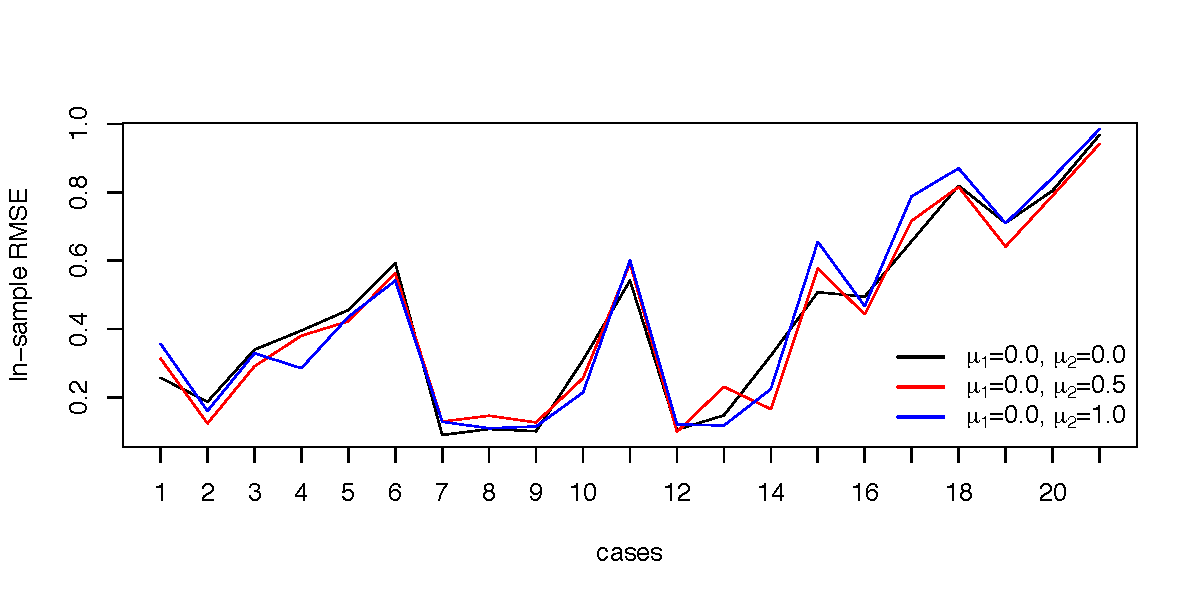
\includegraphics[scale=.8]{RMSEy}
\end{figure}
% #############  end of document##############
\bigskip

\pagebreak




\bigskip 
\end{document}
